\documentclass[WHATMANUAL.tex]{subfiles}

\begin{document}

\chapter{Water-level time-series preparation}

WHAT provides a dynamic graphical environment to explore, validate and apply various corrections to water-level time series. This feature is available in the mode ``computation'' of the tab \emph{Hydrograph} shown in Figure~\ref{fig:tab_hydrograph_computation}.

\begin{figure}[h!]
\centering
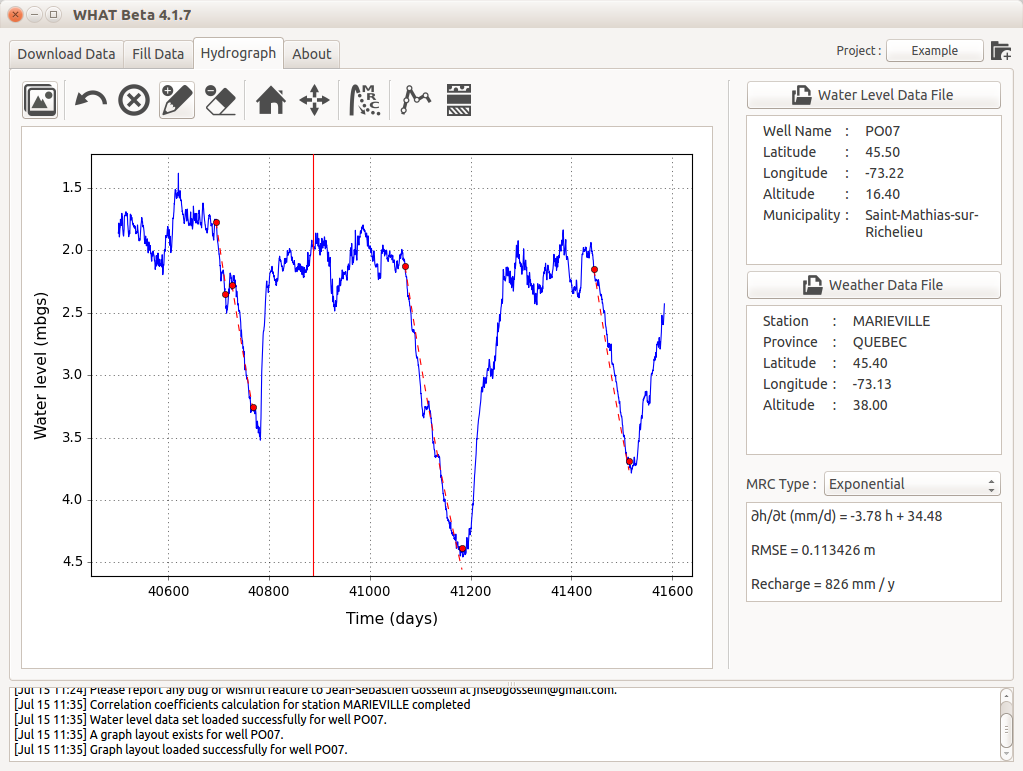
\includegraphics[width=0.75\textwidth]{img/WHAT_Screenshot003}
\caption[Tab ``Download Data''.]{Mode ``Computation'' of the Tab ``Download Data''.}
\label{fig:tab_hydrograph_computation}
\end{figure}

\section{Water Level Format}

Water-level data files can be imported in either in a Microsoft Excel 2003 format (.xls) or a tab-separated values (TSV) text file (``.tsv''). A sample of a water-level data file is provided in the example that is distributed with the software. For the MS Excell format, data must be saved in the first page of the workbook, all the additional pages won't be read by WHAT for performance purposes.

The water-levels must be entered as the height of the water column above the instrument or the submergence depth. This is generally directly the ouput data of vented water-level data loggers (gage pressure transducers). However, non-vented devices record the absolute pressure and their output must be compensated for barometric pressure in order to obtain a measure of the water level elevation. This is done by subtracting the barometric record from the water-level record in order to compute the height of the water column above the instrument. This correction must be made before the water-level data are loaded in WHAT. Some software by the data logger manufacturers are able to do this automatically. Alternately, this can be easily done manually when some theory basics are well understood. This is covered in more detail in Section~X of Chapter~Y.

The measurements must also be accompanied by the times, in the Microsoft Excel numeric time format, at which they were taken. The following link provides a detailed description and analysis of the numeric time format in Microsoft Excel : \url{http://www.lexicon.net/sjmachin/xlrd.html}

\section{Well Configuration and Location Information}

In addition to the data time-series, various information about the well configuration and location are required in the file header for WHAT to work properly. These information are consists in:

\paragraph{Well Name} This is an alphanumeric identifier of the well that must be unique to the project. It can contain any combination of alphabetic and numeric characters, but it is recommended to avoid using the following symbol: \%, ', ", /, \textbackslash. The Well Name is used to store various information about the water level time-series (graph layout, data modification, manual measurements, etc.) and is also used for the generation of the figure labels.

\paragraph{Latitude and Longitude} Location coordinates of the well in decimal degrees. The well location coordinates are used principally for computing the distance between the well and the weather stations and consequently for the generation of the figure labels.

There exists a great online tool for the conversion of geographic units in various format that is provided by the Montana State University. This tool can be accessed at this web address: \url{http://www.rcn.montana.edu/Resources/Converter.aspx}.

\paragraph{Altitude} Altitude of the ground surface relative to the mean see level at the well location in meters above see level. This value is used to convert the water-level measurements when the datum is changed to mean sea level.

\paragraph{Municipality} This field is currently not used in WHAT and is for informational purposes only.

\paragraph{Installation Depth} This is the fixed depth at which water-level data loggers is installed in the well or the piezometer relative to the ground surface. This value is negative if below the ground surface and positive if above.

fixed depth in a well or the piezometer from a stable fixed point called the hanging point, often secured directly to the well casing itself.

\section{Manual Measurements}

Water level manual measurement are imported automatically in WHAT for a given well when


It is necessary to validate the values taken with the automatic logger with manual measurement on a regular basis.

Long-term monitoring of water levels with the use of automatic data loggers can lead to errors if the data are not validated on a regular basis with manual measurements. \cite{freeman_use_2004} provides a good review on possible causes of errors that may be present in data acquired with submersible pressure transducers.

% Text cited as is. Need to reformat it.
The convenience and low maintenance of submersible pressure transducers can lead to long intervals between calibration checks and overconfidence in the reliability of the sensor's data. If checks on the calibration of sensors are not made, data may be erroneous to the point of leading to incorrect hydrologic interpretations.

\section{Water Level Corrections}


The first step is to open the water-level data file in WHAT. This is done simply by clicking on the \emph{Water Level Data File button} that is located at the top of the right side panel of the tab \emph{Hydrograph}. This will open a new window for the selection of a valide water-level data file. Clicking on select will open the file in WHAT.

The second step is to apply corrections obtained from field verification measurements. If the record is faulty due to instrumentation or other problems, corrections usually cannot be applied. In general, a missing or faulty record of ground-water level cannot be estimated reliably.

Four types of corrections can be applied to the record:

datum corrections,
hung-depth corrections,
drift corrections, and calibration corrections. 
Aberration value correction

Use time proration for the first two types of corrections. Apply a datum correction when a change has ocurred to the elevation of the measuring point of the well. Keep a level summary sheet with the site’s permanent file to document reference elevation changes. A hung-depth correction can be applied if the position of the transducer changes relative to its original position, due either to purposeful or accidental raising or lowering of the transducer in the well, or to changes from other causes such as an earthquake. A drift correction—usually a linear proration with time—is applied to compensate for drift in the transducer’s offset calibration. Calibration corrections can be applied either by linear time proration from the time of one calibration to the next, or by starting and ending a constant correction for a specific period of time.

A study of vertical hydraulic head gradients at a well nest in New Hampshire showed that uncorrected data from submersible pressure transducers resulted in an interpretation of reversals in vertical hydraulic-head gradients when none actually occurred (Rosenberry, 1990). In the New Hampshire study, linear adjustment of data based on monthly check measurements would have led to the conclusion that additional water-table fluctuations of up to 0.17 ft occurred when weekly check measurements indicated that sensor drift actually was responsible for those interpreted water-level fluctuations.

Pour l’ensemble des puits, l’écart absolu entre les valeurs des sondes et les mesures manuelles est généralement inférieur à 5 cm.

Pour un même puits, lorsqu'un écart systématique de plus de 5 cm était observé entre les mesures manuelles et les mesures automatiques, une correction des niveaux d’eau a été  appliquée de façon à caler les valeurs obtenues avec les sondes aux mesures manuelles.
Les données aberrantes dans les séries de données ont également été corrigées par interpolation linéaire. C’est données aberrantes sont principalement des mesures qui ont été prises alors que la sonde avait été retirée du puits pour le téléchargement des données, ou encore par du pompage dans les puits lors d’une campagne d’échantillonnage de l’eau.

\chapter{Plotting the data}

\section{Water Level Datum}

If an appropriate value of the altitude of ground surface at the well location is provided in the header of the input file, it will be possible to switch the datum of the water level when plotting the data from Meters Below Ground Surface (mbgs) to Meters Above Sea Level (masl).

In computation mode however, data are always displayed as meter above ground surface, with the values positive when above ground surface and negative when below. Displaying water-level time-series relative to the ground surface is much more useful than relative to mean sea level or as the height of the water column above the instrument.By displaying the value relative to the ground surface, it is easy to see the width of the unsaturated zone water has to pass through to attained the water table and become groundwater recharge. Depth of the unsaturated zone is a major factor in the delai between the response of the water table to precipitation or snowmelt event and it also play a role in the attenuation of the signal. Moreover, knowing the depth of the water level below the ground surface also gives indication about possible evapotranspiration from the water-table and also flood event.

In Layout mode it is possible to plot the water level relative to four different datum:

- meters above ground surface (mags)
- meters below ground surface (mbgs)
- meters above logger (mal)
- meters above see level (masl)

mags and mbgs options have the same reference point, but the vertical axis is inverted in the case of mbgs, with the water level being positive below the ground surface and increasing in value as the depth to the surface increase.





\end{document}